Presentamos aquí los resultados obtenidos para cada ruta.
Para cada ruta elegida presentamos una tabla con los resultados crudos, un gráfico con puntos representando cada salto y un mapa que marca la ruta geográfica que traza la conexión establecida.

En las tablas, notar que incluímos el valor promedio del RTT absoluto de la computadora local hasta cada salto, pero como ya fue mencionado calculamos el ZRTT usando la diferencia de RTT entre un salto y el siguiente.

Para los gráficos usamos el teorema central del limite, dado que tomamos suficientes muestras y las mismas son independientes, la cuenta que efectuamos en el cálculo de ZRTT normaliza los datos. En consecuencia, los mismos pueden ser interpretados como provenientes de una distribucion normal, por lo que decidimos representarlos por encima de la campana de Gauss. Como resultado se puede observar de forma sencilla aquellos saltos que son estadisticamente significativos.

\subsection{Resultados generales}
 En todas nuestras pruebas en valor de $MSS$ obtenido fue de 1452, pero lo calculamos programáticamente antes de cada test para asegurarnos de usar el real en cada sistema utilizado.

 En todos los casos la cantidad de paquetes perdidos fue muy baja (máximo 2 de 50) por lo que no se incluye el valor de $EstimatedPacketLossProbability$ en los resultados específicos de cada ruta.

\subsection{Berkeley}

\begin{tabular}{|c@{\hspace{5ex}}c@{\hspace{5ex}}c@{\hspace{5ex}}c@{\hspace{5ex}}c|}
 \hline
 \rule{0pt}{1.2em}IP & ZRTT & AVG\_RTT & PAIS & CIUDAD\\[0.2em]
 \hline

\rule{0pt}{1.2em} 192.168.2.1  &  0.65 & 35.35 & (Private Address) & (Private Address) \\[0.2em]
\rule{0pt}{1.2em} 200.89.164.137  &  -0.11 & 46.40 & ARGENTINA & Buenos Aires \\[0.2em]
\rule{0pt}{1.2em} 200.89.165.130  &  -0.41 & 43.80 & ARGENTINA & Buenos Aires \\[0.2em]
\rule{0pt}{1.2em} 200.89.165.222  &  -0.27 & 47.29 & ARGENTINA & Buenos Aires \\[0.2em]
\rule{0pt}{1.2em} 208.178.195.205  &  -0.43 & 43.57 & ARGENTINA & Buenos Aires \\[0.2em]
\rule{0pt}{1.2em} 67.17.68.234  &  2.86 & 191.77 & UNITED STATES & Miami \\[0.2em]
\rule{0pt}{1.2em} 4.68.111.121  &  -1.44 & 141.79 & UNITED STATES & Miami \\[0.2em]
\rule{0pt}{1.2em} 4.35.156.66  &  1.07 & 207.65 & UNITED STATES & Los Angeles \\[0.2em]
\rule{0pt}{1.2em} 137.164.11.1  &  -0.2 0& 214.70 & UNITED STATES & Cypress \\[0.2em]
\rule{0pt}{1.2em} 137.164.46.144  &  -0.31 & 216.72 & UNITED STATES & Cypress \\[0.2em]
\rule{0pt}{1.2em} 137.164.50.31  &  -0.34 & 217.22 & UNITED STATES & Cypress \\[0.2em]
\rule{0pt}{1.2em} 128.32.0.37  &  -0.28 & 220.53 & UNITED STATES & Berkeley, CA \\[0.2em]
\rule{0pt}{1.2em} 128.32.0.101  &  -0.46 & 215.66 & UNITED STATES & Berkeley, CA \\[0.2em]
\rule{0pt}{1.2em} 169.229.216.200  &  -0.31 & 217.43 & UNITED STATES & Berkeley, CA \\[0.2em]
\hline
 \end{tabular}

Podemos observar el fenómeno ya mencionado sobre RTTs menores en saltos posteriores.

Efectivamente el salto más grande (de Argentina a EEUU) se corresponde con una diferencia de RTTs sustancial, y esto se ve reflejado en el valor del ZRTT que muestra que se aleja casi tres desvíos standard de la media.

 El valor del throughput estimado para esta ruta fue de 3,864, lo cual por ahora no nos dice mucho pero será relevante al compararlo con las demás rutas.

 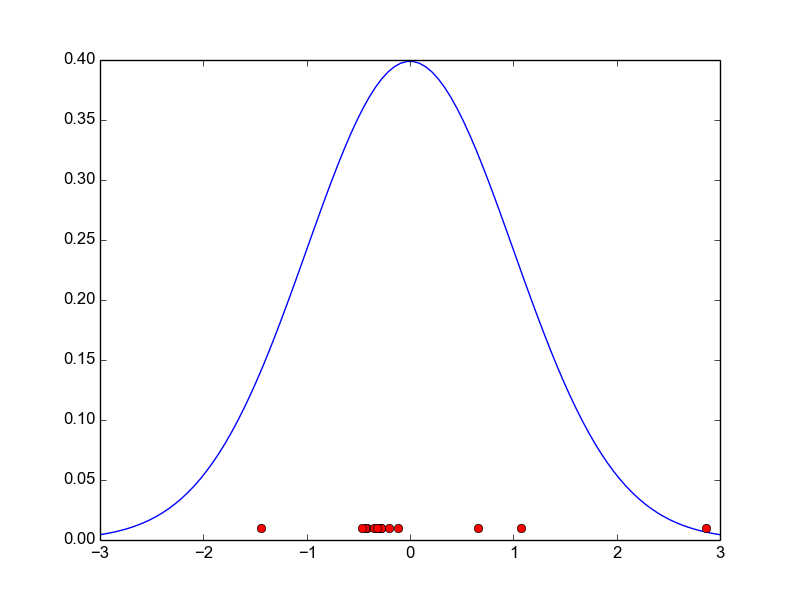
\includegraphics[width=5in]{imgs/berkeley_dist.png}
 \includegraphics[width=5in]{imgs/maps/berkeley.png}


\subsection{Cusat}

\begin{tabular}{|c@{\hspace{5ex}}c@{\hspace{5ex}}c@{\hspace{5ex}}c@{\hspace{5ex}}c|}
 \hline
 \rule{0pt}{1.2em}IP & ZRTT & AVG\_RTT & PAIS & CIUDAD\\[0.2em]
 \hline

\rule{0pt}{1.2em} 192.168.2.1  &  -0.01 & 35.71 & (Private Address) & (Private Address) \\[0.2em]
\rule{0pt}{1.2em} 200.89.164.181  &  -0.33 & 45.44 & ARGENTINA & Buenos Aires \\[0.2em]
\rule{0pt}{1.2em} 200.89.165.150  &  -0.43 & 43.95 & ARGENTINA & Buenos Aires \\[0.2em]
\rule{0pt}{1.2em} 195.22.220.152  &  -0.42 & 44.05 & ARGENTINA & Buenos Aires \\[0.2em]
\rule{0pt}{1.2em} 195.22.216.142  &  1.12 & 213.52 & UNITED STATES & New Orleans \\[0.2em]
\rule{0pt}{1.2em} 195.22.216.142  &  -0.43 & 212.45 & UNITED STATES & New Orleans \\[0.2em]
\rule{0pt}{1.2em} 195.22.195.102  &  1.59 & 434.06 & ITALY & Milano \\[0.2em]
\rule{0pt}{1.2em} 218.248.235.161  &  -1.76 & 286.69 & INDIA & Bangalore \\[0.2em]
\rule{0pt}{1.2em} 210.212.233.50  &  1.10 & 454.65 & INDIA & Cochin \\[0.2em]
\rule{0pt}{1.2em} 210.212.233.50  &  -0.41 & 455.32 & INDIA & Cochin \\[0.2em]
\hline
 \end{tabular}

 En una primera instancia, notamos que el IP 195.22.220.152 fue marcado como Italiano pero su RTT era demasiado bajo. Verificando contra otras bases de localizacion de IP, comprobamos que efectivamente el nodo se encuentra en Argentina, si bien su rango pertenece a Italia, ya que el ISP dueño es una corporacion Italiana.

 Nuevamente vemos una correspondencia entre el salto más largo, trasatlántico esta vez, y la diferencia entre RTTs, reflejada a su vez por el valor de ZRTT. Sin embargo también vemos una diferencia similar entre dos puntos supuestamente cercanos, y una diferencia negativa entre dos puntos supuestamente alejados.

 El valor del throughput estimado para esta ruta fue de 3,203. Comparándolo con el anterior, que el valor absoluto de RTT de la ruta sea mucho mayor afecta directamente al throughput obtenido.

 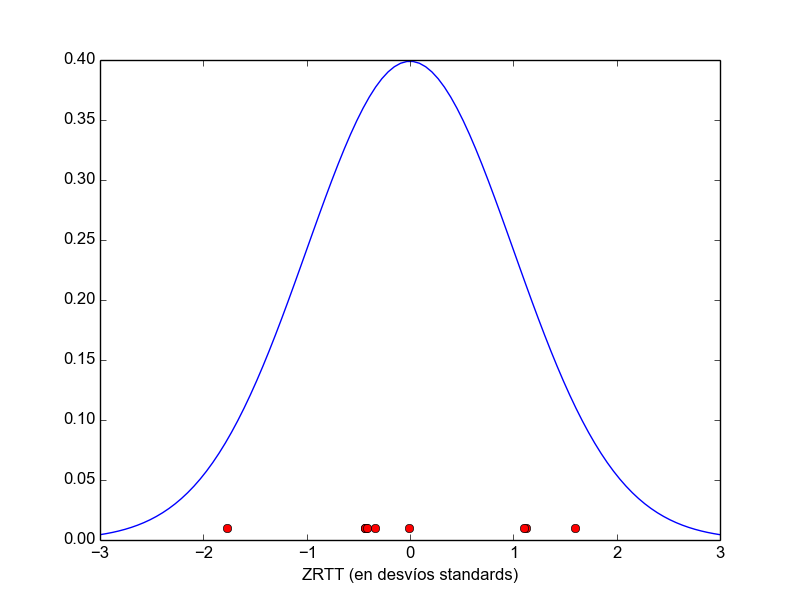
\includegraphics[width=5in]{imgs/cusat_dist.png}
 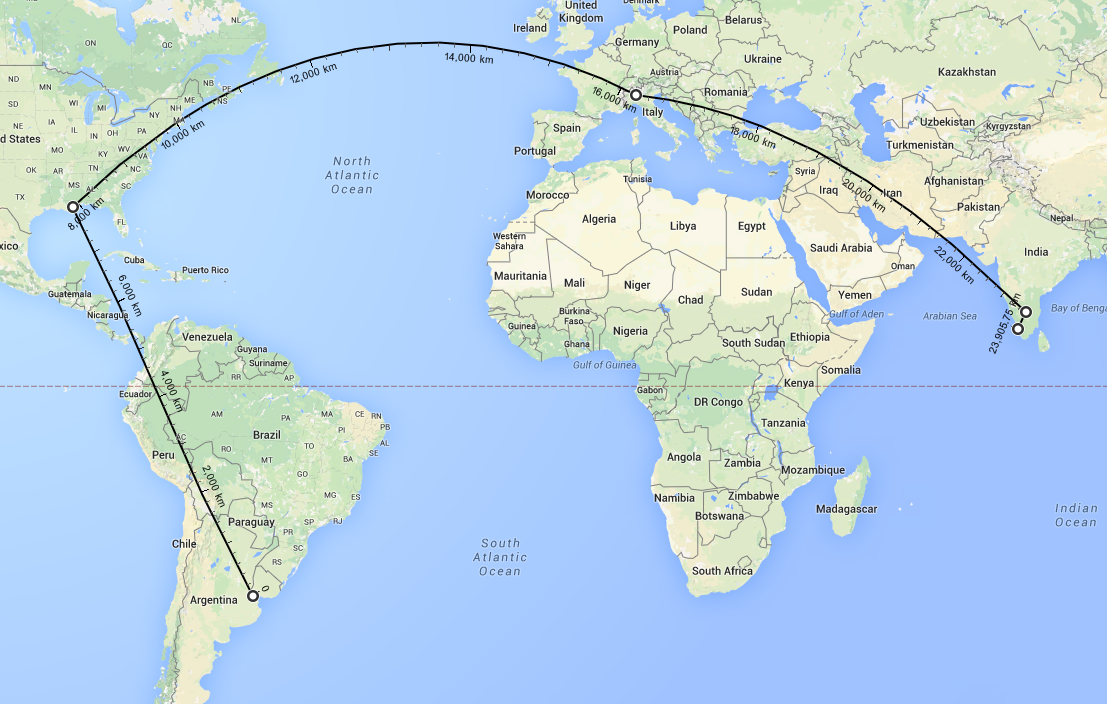
\includegraphics[width=5in]{imgs/maps/cusat.png}

\subsection{Islandia}

\begin{tabular}{|c@{\hspace{5ex}}c@{\hspace{5ex}}c@{\hspace{5ex}}c@{\hspace{5ex}}c|}
 \hline
 \rule{0pt}{1.2em}IP & ZRTT & AVG\_RTT & PAIS & CIUDAD\\[0.2em]
 \hline

\rule{0pt}{1.2em} 192.168.2.1  &  0.53 & 37.3 & (Private Address) & (Private Address) \\[0.2em]
\rule{0pt}{1.2em} 200.89.164.153  &  -0.24 & 45.36 & ARGENTINA & Buenos Aires \\[0.2em]
\rule{0pt}{1.2em} 200.89.165.130  &  -0.42 & 44.90 & ARGENTINA & Buenos Aires \\[0.2em]
\rule{0pt}{1.2em} 200.89.165.222  &  -0.36 & 47.18 & ARGENTINA & Buenos Aires \\[0.2em]
\rule{0pt}{1.2em} 208.178.195.205  &  -0.48 & 43.77 & ARGENTINA & Buenos Aires \\[0.2em]
\rule{0pt}{1.2em} 67.16.139.18  &  3.11 & 211.71 & UNITED STATES & Miami \\[0.2em]
\rule{0pt}{1.2em} 213.248.76.189  &  -1.33 & 168.31 & UNITED STATES & Miami \\[0.2em]
\rule{0pt}{1.2em} 62.115.136.204  &  0.28 & 201.46 & UNITED STATES & Ashburn \\[0.2em]
\rule{0pt}{1.2em} 213.155.133.229  &  -0.46 & 199.20 & UNITED STATES & Ashburn \\[0.2em]
\rule{0pt}{1.2em} 213.248.85.174  &  1.01 & 267.33 & UNITED STATES & Los Angeles \\[0.2em]
\rule{0pt}{1.2em} 109.105.97.140  &  -0.35 & 270.48 & SWEDEN & Stockholm \\[0.2em]
\rule{0pt}{1.2em} 109.105.97.42  &  0.53 & 315.58 & SWEDEN & Stockholm \\[0.2em]
\rule{0pt}{1.2em} 109.105.102.2  &  -0.59 & 307.25 & SWEDEN & Stockholm \\[0.2em]
\rule{0pt}{1.2em} 130.208.17.106  &  -0.38 & 308.99 & ICELAND & Reykjavik \\[0.2em]
\rule{0pt}{1.2em} 130.208.18.174  &  -0.29 & 314.75 & ICELAND & Reykjavik \\[0.2em]
\rule{0pt}{1.2em} 130.208.165.207  &  -0.53 & 309.26 & ICELAND & Reykjavik \\[0.2em]
\hline
 \end{tabular}

 Una vez más el valor del ZRTT es consistente con el salto grande entre Argentina y EEUU, pero eso no parece ocurrir con el que hay entre EEUU y Suecia.
 Si bien se observa un salto en tiempos en la ruta de costa a costa de EEUU, luego el tiempo para llegar hasta Suecia el salto siguiente, es muy bajo.
 No hemos podido terminar de detectar a qué se deben estas inconsistencias.


 El throughput estimado para esta ruta fue de 4,632, el mayor de todas las rutas. Entendemos que tiene que ver con el bajo RTT obtenido y con una buena calidad de la conexión, con nula pérdidas de paquetes.

 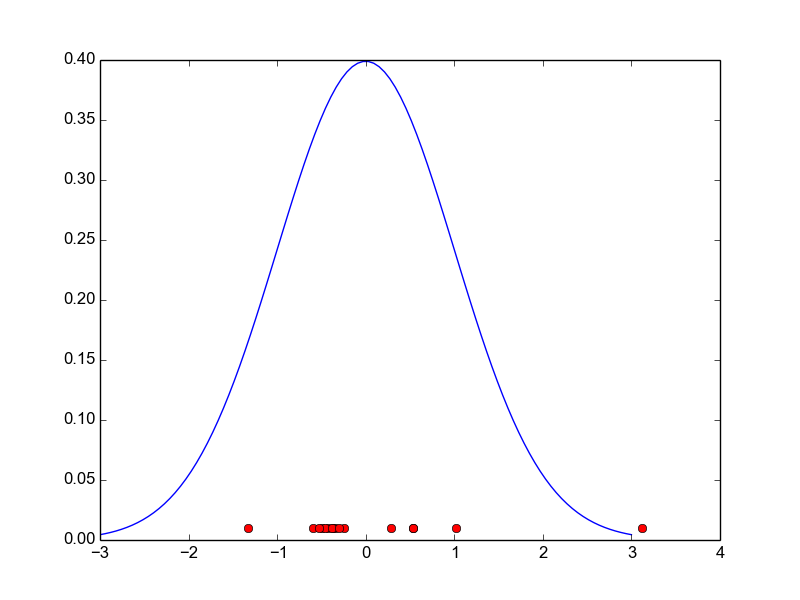
\includegraphics[width=5in]{imgs/iceland_dist.png}
 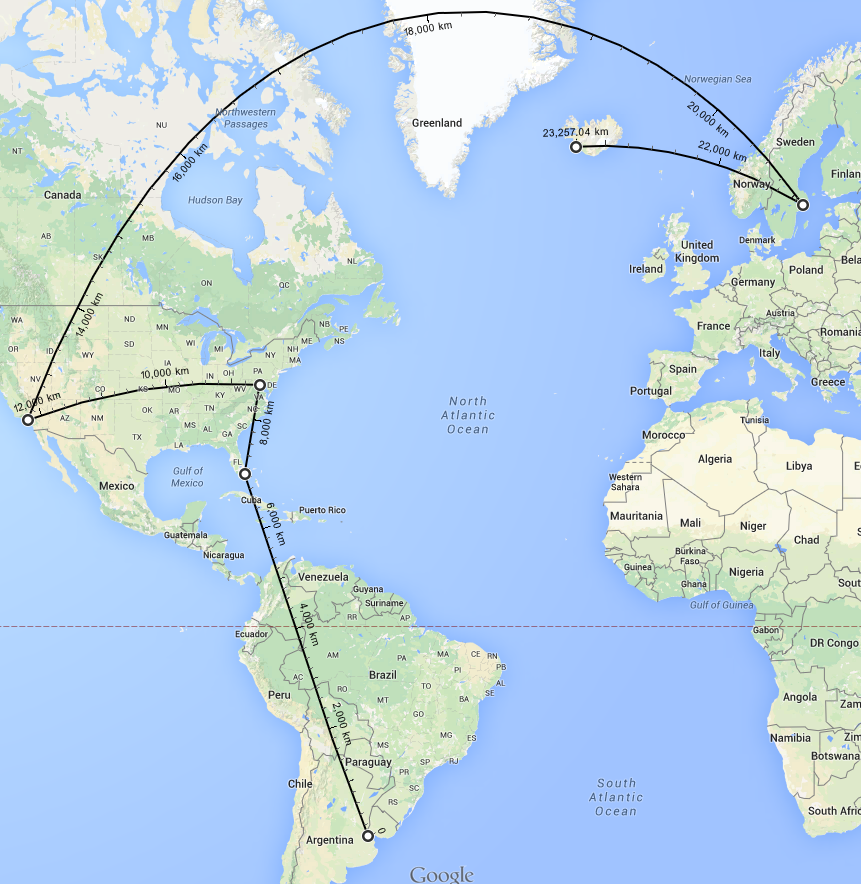
\includegraphics[width=5in]{imgs/maps/iceland2.png}


 Inicialmente los datos de geolocalización de esta ruta eran los que se muestran a continuación, que indicaban todos nodos en Miami hasta el salto a Suecia, pero esto no resultaba certero ya que entre los saltos en estados unidos había una variación muy alta (la correspondiente al salto hasta Los Angeles)

 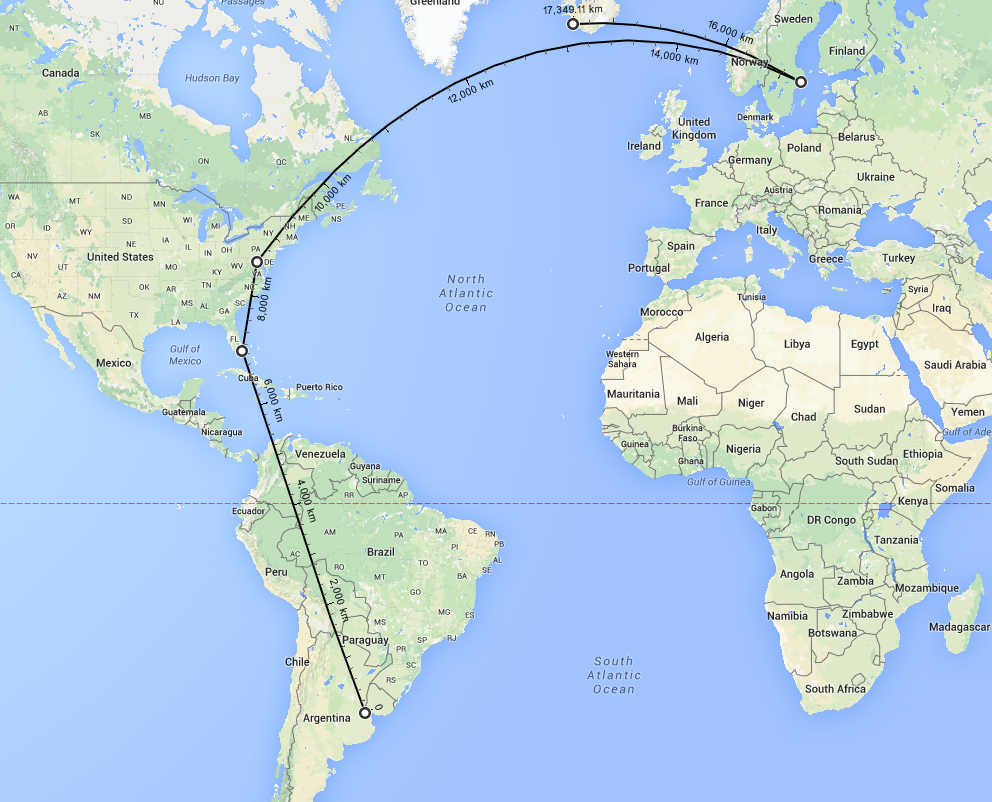
\includegraphics[width=5in]{imgs/maps/iceland.png}

\subsection{Perm}

\begin{tabular}{|c@{\hspace{5ex}}c@{\hspace{5ex}}c@{\hspace{5ex}}c@{\hspace{5ex}}c|}
 \hline
 \rule{0pt}{1.2em}IP & ZRTT & AVG\_RTT & PAIS & CIUDAD\\[0.2em]
 \hline

\rule{0pt}{1.2em} 192.168.2.1  &  0.36 & 35.15 & (Private Address) & (Private Address) \\[0.2em]
\rule{0pt}{1.2em} 200.89.166.161  &  -0.30 & 45.49 & ARGENTINA & Buenos Aires \\[0.2em]
\rule{0pt}{1.2em} 200.89.165.130  &  -0.51 & 44.81 & ARGENTINA & Buenos Aires \\[0.2em]
\rule{0pt}{1.2em} 200.89.165.222  &  -0.46 & 46.45 & ARGENTINA & Buenos Aires \\[0.2em]
\rule{0pt}{1.2em} 208.178.244.213  &  -0.52 & 45.05 & ARGENTINA & Buenos Aires \\[0.2em]
\rule{0pt}{1.2em} 67.17.75.66  &  2.54 & 205.42 & UNITED STATES & Miami \\[0.2em]
\rule{0pt}{1.2em} 4.68.111.121  &  -1.06 & 175.47 & UNITED STATES & Miami \\[0.2em]
\rule{0pt}{1.2em} 4.69.158.245  &  1.89 & 301.85 & SWEDEN & Stockholm \\[0.2em]
\rule{0pt}{1.2em} 4.69.158.245  &  -0.42 & 305.45 & SWEDEN & Stockholm \\[0.2em]
\rule{0pt}{1.2em} 213.242.110.198  &  -0.26 & 317.85 & SWEDEN & Stockholm \\[0.2em]
\rule{0pt}{1.2em} 194.85.40.229  &  -0.29 & 328.49 & RUSSIAN FEDERATION & Saint Petersburg \\[0.2em]
\rule{0pt}{1.2em} 194.226.194.22  &  0.01 & 355.20 & RUSSIAN FEDERATION & Saint Petersburg \\[0.2em]
\rule{0pt}{1.2em} 212.192.80.57  &  -0.57 & 351.03 & RUSSIAN FEDERATION & Perm \\[0.2em]
\rule{0pt}{1.2em} 212.192.64.44  &  -0.37 & 357.50 & RUSSIAN FEDERATION & Perm \\[0.2em]
\hline
 \end{tabular}

 Nuevamente hace falta ``pasar por'' Miami para llegar a Europa, y una vez más el ZRTT es consistente con este salto.
 Inicialmente esta ruta fue complicada de analizar, ya que obteníamos un salto transatlántico sorprendentemente corto.
 Luego de corroborar mejor nuestras fuentes de geolocalización IP lo mismo cobró más coherencia observando que el salto transatlántico entre Estados Unidos y Suecia era lo que tenía el ZRTT alto.


 El throughput estimado para esta ruta fue de 3,923, nuevamente un valor comparativamente alto aunque no tanto como con el enlace con Islandia.

 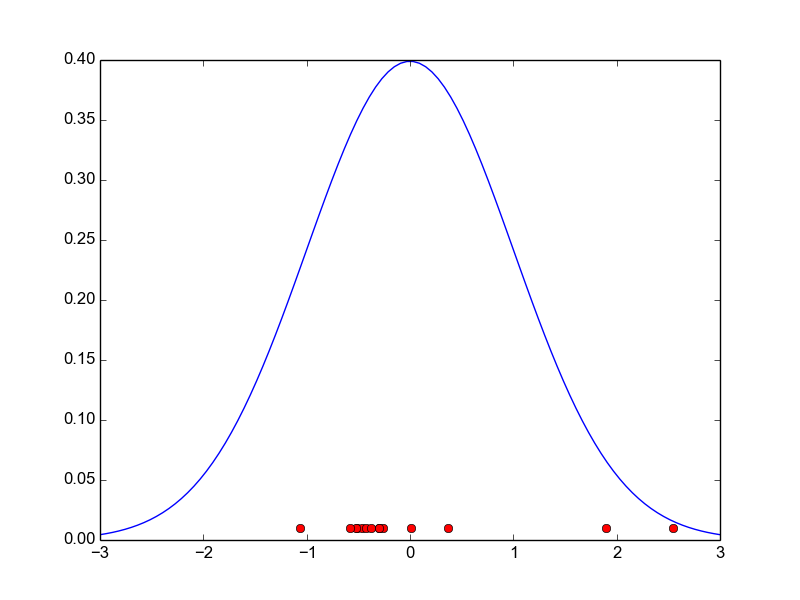
\includegraphics[width=5in]{imgs/perm_dist.png}
 \includegraphics[width=5in]{imgs/maps/perm.png}

\subsection{Pretoria}

\begin{tabular}{|c@{\hspace{5ex}}c@{\hspace{5ex}}c@{\hspace{5ex}}c@{\hspace{5ex}}c|}
 \hline
 \rule{0pt}{1.2em}IP & ZRTT & AVG\_RTT & PAIS & CIUDAD\\[0.2em]
 \hline

\rule{0pt}{1.2em} 192.168.2.1  &  0.42 & 35.29 & (Private Address) & (Private Address) \\[0.2em]
\rule{0pt}{1.2em} 200.89.164.177  &  -0.20 & 45.07 & ARGENTINA & Buenos Aires \\[0.2em]
\rule{0pt}{1.2em} 200.89.165.130  &  -0.38 & 44.64 & ARGENTINA & Buenos Aires \\[0.2em]
\rule{0pt}{1.2em} 200.89.165.222  &  -0.36 & 45.49 & ARGENTINA & Buenos Aires \\[0.2em]
\rule{0pt}{1.2em} 208.178.195.205  &  -0.43 & 42.76 & ARGENTINA & Buenos Aires\\[0.2em]
\rule{0pt}{1.2em} 67.17.106.162  &  2.64 & 211.71 & UNITED STATES & Miami \\[0.2em]
\rule{0pt}{1.2em} 154.54.13.61  &  -1.14 & 168.90 & UNITED STATES & Atlanta \\[0.2em]
\rule{0pt}{1.2em} 154.54.24.233  &  -0.37 & 169.24 & UNITED STATES & Atlanta \\[0.2em]
\rule{0pt}{1.2em} 154.54.24.197  &  -0.13 & 183.11 & UNITED STATES & Atlanta \\[0.2em]
\rule{0pt}{1.2em} 154.54.31.110  &  -0.20 & 193.00 & UNITED STATES & Atlanta \\[0.2em]
\rule{0pt}{1.2em} 154.54.7.26  &  -0.28 & 198.41 & UNITED STATES & Chicago \\[0.2em]
\rule{0pt}{1.2em} 154.54.31.118  &  -0.39 & 197.44 & UNITED STATES & New York \\[0.2em]
\rule{0pt}{1.2em} 154.54.30.186  &  1.13 & 282.38 & UNITED KINGDOM & London \\[0.2em]
\rule{0pt}{1.2em} 130.117.50.201  &  -0.44 & 278.99 & ITALY & Milan \\[0.2em]
\rule{0pt}{1.2em} 154.54.38.190  &  -0.22 & 287.66 & UNITED KINGDOM & London \\[0.2em]
\rule{0pt}{1.2em} 149.14.80.210  &  -0.01 & 308.23  & UNITED KINGDOM & London \\[0.2em]
\rule{0pt}{1.2em} 196.32.209.50  &  -0.66 & 292.33 & SOUTH AFRICA & Cape Town \\[0.2em]
\rule{0pt}{1.2em} 196.32.209.117  &  3.08 & 485.75 & SOUTH AFRICA & Cape Town \\[0.2em]
\rule{0pt}{1.2em} 155.232.6.86  &  -0.63 & 471.57 & SOUTH AFRICA & Wynberg \\[0.2em]
\rule{0pt}{1.2em} 155.232.6.29  &  -0.07 & 488.65 & SOUTH AFRICA & Wynberg \\[0.2em]
\rule{0pt}{1.2em} 155.232.6.138  &  -0.66 & 472.79 & SOUTH AFRICA & Wynberg \\[0.2em]
\rule{0pt}{1.2em} 137.215.99.2  &  -0.17 & 484.43 & SOUTH AFRICA & Pretoria \\[0.2em]
\rule{0pt}{1.2em} 137.215.10.70  &  -0.45 & 480.05 & SOUTH AFRICA & Pretoria \\[0.2em]
\hline
 \end{tabular}

 Por lejos nuestra ruta más larga, lo primero que notamos es que a pesar de la relativa cercanía geográfica, para conectar Sudamérica con África hace falta pasar por continentes del norte (y una vez más por Miami, casi una constante de todas las rutas elegidas). Esta vez el salto trasatlántico sí tiene un ZRTT grande (más de un desvío standard) y el otro salto significativo es dentro de Cape Town, en Sudáfrica, cosa extraña.
 Creemos puede tener que ver con algún tipo error de geolocalización, aunque en varias bases de datos con fechas diferentes de actualización la localización resultaba consistente.
 La demora inducida en estos saltos pareciera muy grande para tratarse de demoras de encolamiento o situaciones similares en loops locales de Sudáfrica.

 Además, hemos re-analizado la diferencia entre los hosts 196.32.209.50 y 196.32.209.117 por separado, ya que ambos responden al ping, con herramientas adicionales como para verificar mejor esta situación. Estos checkeos nos dieron resultados similares a los calculados por nuestra herramienta. Aproximadamente 175ms de diferencia.


 El throughput estimado para esta ruta fue de 3,030, el más bajo de las rutas usadas. Entendemos que tiene que ver con la gran distancia física que recorre la conexión trazada y su consiguiente RTT mayor a las demás rutas.

 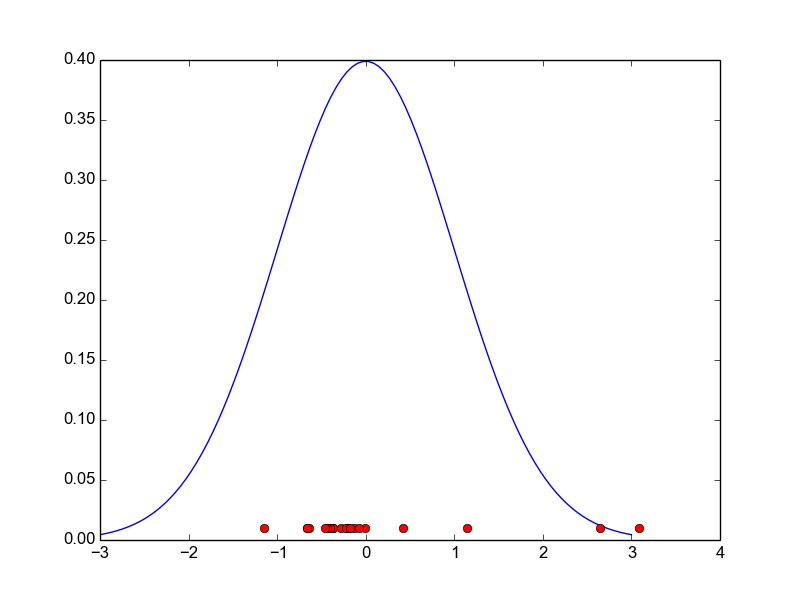
\includegraphics[width=5in]{imgs/pretoria_dist.png}
 \includegraphics[width=5in]{imgs/maps/pretoria.png}
